\begin{frame}{Who? - Lecturers}
	%Melanie Bianca Sigl
	\begin{columns}[T]
		\begin{column}{0.2\textwidth}
			\vspace{-1em}
			\begin{figure}[T]
				\centering
				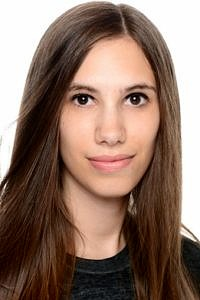
\includegraphics[width=0.55\textwidth]{img/melanie_b_sigl.jpg}
			\end{figure}
		\end{column}
		\begin{column}{0.8\textwidth}
			\textbf{Melanie Bianca Sigl, M.Sc.}
			\begin{itemize}
				\item External Ph.D. candidate at Computer Science 6 (Data Management)
				\item Senior Consultant at PRODATO Integration Technology GmbH
				\item E-Mail: \texttt{\href{mailto:melanie.sigl@fau.de}{melanie.sigl@fau.de}}
				\item Website: \url{https://www.cs6.tf.fau.eu/person/melanie-sigl/}
			\end{itemize}
		\end{column}
	\end{columns}

	\vspace{2em}

	%Dominik Probst
	\begin{columns}[T]
		\begin{column}{0.2\textwidth}
			\vspace{-1em}
			\begin{figure}[t]
				\centering
				\includegraphics[width=0.55\textwidth]{img/dominik_probst.jpg}
			\end{figure}
		\end{column}
		\begin{column}{0.8\textwidth}
			\textbf{Dominik Probst, M.Sc.}
			\begin{itemize}
				% Following the guidelines for our business cards without "Chair of"
				\item Ph.D. candidate
				\item Computer Science 6 (Data Management)
				\item E-Mail: \texttt{\href{mailto:dominik.probst@fau.de}{dominik.probst@fau.de}}
				\item Website: \url{https://www.cs6.tf.fau.de/person/dominik-probst/}
			\end{itemize}
		\end{column}
	\end{columns}
\end{frame}

\begin{frame}{For whom? - Courses of Study}
	% Study programs
	\begin{itemize}
		\item \textbf{Knowledge Discovery in Databases with Exercise (KDDmUe)} - 5 ECTS
		      \begin{itemize}
			      \item B.Sc. Data Science
			      \item M.Sc. Computer Science
			      \item {\color{gray} Possibly other courses of study (clarify with your examination office)}
		      \end{itemize}
		\item \textbf{Knowledge Discovery in Databases (KDD)} - 2.5 ECTS
		      \begin{itemize}
			      \item M.Sc. Information and Communication Technology
			      \item M.Sc. Medical Engineering
		      \end{itemize}
	\end{itemize}

	\begin{alertblock}{Important: KDDmUe Replaces KDDTAS in B.Sc. Data Science!}
		Although the module KDDTAS is listed in the examination regulations of B.Sc. Data Science, it is no longer offered by us. Module KDDmUe is the replacement for it and is recognized by us accordingly.
	\end{alertblock}
\end{frame}

\begin{frame}{For whom? - Prerequisites}
	%Prerequisites
	\begin{itemize}
		\item \textbf{Mandatory requirements:}
		      \begin{itemize}
			      \item Successful completion of the module \glqq Konzeptionelle Modellierung\grqq~(KonzMod)
		      \end{itemize}
		\item \textbf{Useful prerequisites:}
		      \begin{itemize}
			      \item Successful completion of the module \glqq Implementierung von Datenbanksystemen\grqq~(IDB)
			      \item Experience with:
			            \begin{itemize}
				            \item Python
				            \item Jupyter Notebooks
				            \item Numpy
				            \item Pandas
				            \item Algorithms
				            \item Data structures
			            \end{itemize}
		      \end{itemize}
	\end{itemize}

\end{frame}


\begin{frame}{What? - Goal and Topics}
	% Goal of the lecture
	\begin{itemize}
		\item \textbf{Goal of the module:}
		      \begin{itemize}
			      \item Introduce you to the principles of data mining. \\
			            $\Rightarrow$ This is the core of knowledge discovery in databases
		      \end{itemize}
		\item \textbf{Topics in the lecture:}
		      \vspace*{-1\multicolsep}
		      \begin{multicols}{2}
			      \begin{enumerate}
				      \item Introduction {\color{gray} - D. Probst}
				      \item Data {\color{gray} - M. B. Sigl}
				      \item Preprocessing {\color{gray} - D. Probst}
				      \item Data Warehousing {\color{gray} - M. B. Sigl}
				      \item Mining Frequent Patterns {\color{gray} - D. Probst}
				      \item Classification {\color{gray} - M. B. Sigl}
				      \item Cluster Analysis {\color{gray} - D. Probst}
				      \item Outlier Analysis {\color{gray} - M. B. Sigl}
				      \item {\color{gray}Guest lecture by Friedrich-Claus Grüber (Siemens Energy)}
			      \end{enumerate}
		      \end{multicols}
		      \vspace*{-1\multicolsep}
		\item \textbf{Topics in the exercise:}
		      \vspace*{-1\multicolsep}
		      \begin{multicols}{2}
			      \begin{enumerate}
				      \item Introduction to python and pandas {\color{gray}optional}
				      \item Data Analysis and Data Preprocessing
				      \item Frequent Patterns
				      \item Classification
				      \item Clustering
				      \item Outlier
			      \end{enumerate}
		      \end{multicols}
		      \
	\end{itemize}
\end{frame}

\begin{frame}{What? - Exam}
	% Exam
	\begin{itemize}
		\item \textbf{Knowledge Discovery in Databases with Exercise (KDDmUe)} - {\color{faugray}Written Exam}
		      \begin{itemize}
			      \item Duration: 90 minutes
			      \item Questions about both lecture and exercise content
			      \item Language: English
		      \end{itemize}
		\item \textbf{Knowledge Discovery in Databases (KDD)} - {\color{faugray}Oral Exam}
		      \begin{itemize}
			      \item Duration: 30 minutes
			      \item Questions about lecture content only
			      \item Language: English or German
		      \end{itemize}
	\end{itemize}
	\begin{alertblock}{Important: Do Not Forget to Register!}
		Without exception, we can only examine participants who have also registered for this exam at the examination office. Please note the information of the examination office as to when registration takes place in this semester.
	\end{alertblock}
\end{frame}

\begin{frame}{What? - Literature}
	% Literature
	\begin{itemize}
		\item \textbf{This lecture is based on the book by \citeauthor{han2011}:}
		      \begin{itemize}
			      \item \fullcite{han2011}
			      \item {\color{faugray}Copies are available at the Science and Technology Branch Library (TNZB).}
			      \item Lecture slides are based on slides provided by Jiawei Han with modifications by Prof. Dr.-Ing. Klaus Meyer-Wegener and Luciano Melodia.
			      \item Lecture slides have been modified and extended since then.
		      \end{itemize}
		\item \textbf{Further books on this topic include, but not limited to:}
		      \begin{itemize}
			      \item \fullcite{geron2017}
			      \item \fullcite{du2010}
			      \item \fullcite{witten2016}
		      \end{itemize}
	\end{itemize}
\end{frame}

\begin{frame}{When? - Dates}
	% Dates
	\begin{itemize}
		\item \textbf{Lecture} - Start in Calendar Week 17 (Today)
		      \begin{itemize}
			      \item Monday, 10:15 - 11:45 (Online via Zoom) \\
			            {\color{gray}Lecturers: M. B. Sigl and D. Probst}
		      \end{itemize}
		\item \textbf{Exercises} - Start in Calendar Week 18
		      \begin{itemize}
			      \item Wednesday, 14:15 - 15:45 (H8) \\
			            {\color{gray}Tutor: D. Probst}
			      \item Friday, 16:15 - 17:45 (Online via Zoom) \\
			            {\color{gray}Tutors: M. B. Sigl and D. Probst}
		      \end{itemize}
	\end{itemize}

	\begin{block}{Registration for Exercises}
		Registration for exercises is mandatory to ensure an appropriate support to questions regarding setting of exercises should they arise.
			{\color{faured}Registration opens at April 25th, 18:00 o'clock via StudOn.}
	\end{block}
\end{frame}

\begin{frame}{When? - Preliminary Schedule}
	% Schedule
	\footnotesize
	\centering
	\begin{tabular}{|p{4em}|p{21em}|p{21em}|}
		\hline
		\rowcolor{faugray!62}\textbf{Calendar Week} & \textbf{Lecture}                                                            & \textbf{Exercise}                                            \\ \hhline{*{3}{:=}:}
		\cellcolor{faugray!25}17                    & Prologue + Introduction                                                     & \cellcolor{gray!50}                                          \\ \hline
		\cellcolor{faugray!25}18                    & Data                                                                        &
		Introduction to python \& pandas {\color{gray}(optional)}                                                                                                                                \\ \hline
		\cellcolor{faugray!25}19                    & \multirow{2}{*}{Preprocessing}                                              & \multirow{3}{*}[-0.6em]{Data Analysis \& Data Preprocessing} \\
		\cellcolor{faugray!25}20                    &                                                                             &                                                              \\ \hhline{|--|~|}
		\cellcolor{faugray!25}21                    & \textcolor{gray}{Guest lecture (Siemens Energy)} +\newline Data Warehousing &                                                              \\ \hline
		\cellcolor{faugray!25}22                    & Frequent Pattern                                                            & Frequent Pattern                                             \\ \hline
		\cellcolor{faugray!25}23                    & \multicolumn{2}{c}{\cellcolor{gray!50}}                                                                                                    \\ \hline
		\cellcolor{faugray!25}24                    & Frequent Pattern                                                            & Frequent Pattern                                             \\ \hline
		\cellcolor{faugray!25}24                    & \multirow{2}{*}{Classification}                                             & \multirow{2}{*}{Classification}                              \\
		\cellcolor{faugray!25}25                    &                                                                             &                                                              \\ \hline
		\cellcolor{faugray!25}26                    & \multirow{2}{*}{Cluster Analysis}                                           & \multirow{2}{*}{Clustering}                                  \\
		\cellcolor{faugray!25}27                    &                                                                             &                                                              \\ \hline
		\cellcolor{faugray!25}28                    & \multirow{2}{*}{\shortstack[l]{Outlier Analysis +                                                                                          \\ \textcolor{gray}{Current Research at CS6 and Exam Q\&A}}}                                           & Outlier                                     \\ \hhline{|-|~|-|}
		\cellcolor{faugray!25}29                    &                                                                             & \cellcolor{gray!50}                                          \\ \hline
	\end{tabular}
\end{frame}

\begin{frame}{Where? - StudOn}
	% StudOn
	\begin{columns}
		\begin{column}{0.7\textwidth}
			\begin{itemize}
				\item Register at: \url{https://www.studon.fau.de/crs4353407_join.html}
				\item Main source for resources. E.g.:
				      \begin{itemize}
					      \item Zoom access data
					      \item Lecture slides
					      \item Exercise sheets
					      \item Forum
				      \end{itemize}
				\item Membership required to receive important updates on KDD by mail
				\item Questions should be asked here (StudOn Forum)

			\end{itemize}
		\end{column}
		\begin{column}{0.3\textwidth}
			\begin{center}
				\qrcode{https://www.studon.fau.de/crs4353407_join.html}
			\end{center}
		\end{column}
	\end{columns}

\end{frame}


\begin{frame}{Where? - GitHub}
	% GitHub
	\begin{columns}
		\begin{column}{0.7\textwidth}
			\begin{itemize}
				\item Public repository at: \url{https://github.com/FAU-CS6/KDD}
				\item Version control of our resources including:
				      \begin{itemize}
					      \item Lecture slides
					      \item Exercise sheets
				      \end{itemize}
			\end{itemize}
		\end{column}
		\begin{column}{0.3\textwidth}
			\begin{center}
				\qrcode{https://github.com/FAU-CS6/KDD}
			\end{center}
		\end{column}
	\end{columns}
	\vspace{5mm}
	\begin{exampleblock}{Help Appreciated: Error Corrections}
		Even though we strive for error-free lecture slides and practice sheets, there is still the possibility  that errors have slipped in. You can help us mitigate these inaccuracies: Mail us, or better yet, in the case you have a GitHub account, open up a GitHub issue or create a pull request. Any pointers to errors are very much appreciated.
	\end{exampleblock}

\end{frame}
